The purpose of this section is to answer both the checkpoint and report
questions of the HTTP lab sessions, as well as discuss any relevant results
obtained during the experiences.

\subsection{HTTP GET/response}
After starting Wireshark and choosing a network device, several live packets
are displayed, along with their source and destination IPs, the protocol used,
length, and summarized information. For this experience, we applied a filter to
focus only on HTTP messages.

After visiting the requested url on our browser, two packets were immediately
displayed.

\begin{figure}[htbp]
    \centering
    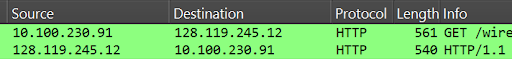
\includegraphics[width=1\linewidth]{img/1.png}
    \caption{Captured packets}\label{fig:1}
\end{figure}

Clicking a packet reveals a viewport on the lower side of the screen, which
displays the information contained in the HTTP message. At a glance, we can see
that our browser used HTTP 1.1 for its request.

\begin{figure}[htbp]
    \centering
    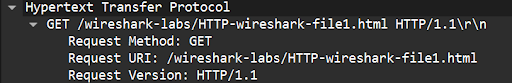
\includegraphics[width=1\linewidth]{img/2.png}
    \caption{HTTP version (request)}\label{fig:2}
\end{figure}

Similarly, clicking the response packet displays that the same HTTP version was
used by the server when sending its response.

\begin{figure}[htbp]
    \centering
    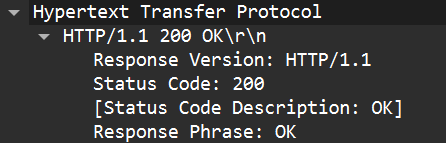
\includegraphics[width=1\linewidth]{img/3.png}
    \caption{HTTP version (response)}\label{fig:3}
\end{figure}

After checking the HTTP versions, we can find both source and destination IPs,
i.e our computer and the server, on the top viewport of the screen, as shown in
Figure~\ref{fig:1}. Our IP is 10.100.230.91, and the IP corresponding to
gaia.cs.umass.edu is 128.119.245.12.\\

The status code returned from the server is 200, as displayed in
Figure~\ref{fig:3}.\\

After checking the section just below the information display in Figure 3, we
can see that the requested HTML file was last modified at 27/08, 5:59.01, GMT
time zone. This is just moments before the time of request, which makes sense
as the server is configured to change the HTML file's modification time each
minute.

\begin{figure}[htbp]
    \centering
    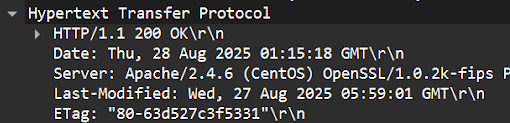
\includegraphics[width=1\linewidth]{img/4.png}
    \caption{Last-Modified}\label{fig:4}
\end{figure}

In a different section, we can see that the length of the response is 526
bytes, while the HTML file itself accounts for 128 bytes of the total length.

\begin{figure}[htbp]
    \centering
    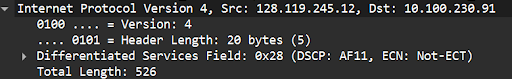
\includegraphics[width=1\linewidth]{img/5.png}
    \caption{Response length}\label{fig:5}
\end{figure}

\begin{figure}[htbp]
    \centering
    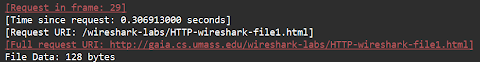
\includegraphics[width=1\linewidth]{img/6.png}
    \caption{HTML length}\label{fig:6}
\end{figure}

The lower viewport, that is, the packet listing window, we can see the headers
used by both requests and responses. Alternatively, this information can also
be seen in the raw data window, so we can conclude that Wireshark shows all of
the available information in the raw data section.

\subsection{HTTP conditional GET/response}
a

\subsection{Retrieving long documents}

\subsection{Report Specific Research}

\subsubsection{HTTP/2}
h2

\subsubsection{HTTP/3}
h3

\subsubsection{HTTP/Secure}
hs

\subsection{HTML documents with embedded objects}
emb

\subsection{HTTP authentication}
auth